% questions.tex —— 1958 年·江苏卷 · 题目内容片段（无答案）
% 由 tools/generate_projects.py 依来源总账自 1958/1958_江苏_数学真题_试题.md 生成，勿手改（改源 MD 后重跑）


\begin{question}
\gkti{1}解下列各题：

（1） 解方程 $\lg(x+7)-\lg(x+1)=\lg(x+3)$；

（2） 解方程 $\sin 10^{x}=\dfrac{1}{2}$；

（3） 设 $\tan\dfrac{\theta}{2}=t$，求证：$\tan\theta=\dfrac{2t}{1-t^{2}}$，$\sin\theta=\dfrac{2t}{1+t^{2}}$，$\cos\theta=\dfrac{1-t^{2}}{1+t^{2}}$。

\end{question}
\begin{question}
\gkti{2}解方程 $\sin x+\sqrt{3}\cos x=2$。

\end{question}
\begin{question}
\gkti{3}已知正六棱锥底边长为 $a$，高为 $h$，求侧面积。

\end{question}
\begin{question}
\gkti{4}已知长方体三度的和为 $a+b+c=13$，对角线长为 $\sqrt{65}$，求全面积。

\Needspace{0.4\textheight}
\end{question}
\begin{question}
\gkti{5}已知 $AB$ 为圆的直径，$DC$ 为圆的弦，四边形 $ABCD$ 内接于圆。

（1） 求证：$AC\cdot DB=AB\cdot DC+AD\cdot CB$；

（2） 求证：直径 $AB$ 为方程 $x^{3}-(a^{2}+b^{2}+c^{2})x-2abc=0$ 的根。
\nopagebreak[4]
\begin{center}% 1958 年江苏卷第 5 题：圆内接四边形 ABCD（AB 为水平直径，D、C 在上半圆，D 约 115°、C 约 56° 方向），连 AD、DC、CB 与对角线 AC、DB；源卷图无顶点圆点、无圆心标记，故不标（按源卷布局）
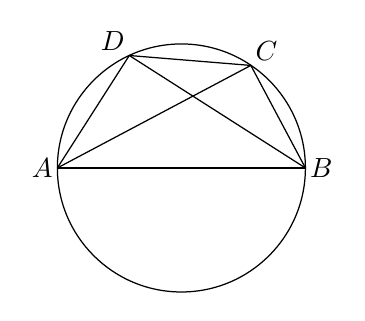
\begin{tikzpicture}[scale=1.05, line width=0.45pt,
  every node/.style={inner sep=1.5pt}]
  \coordinate (A) at (-1.5,0);
  \coordinate (B) at (1.5,0);
  \coordinate (D) at (-0.63,1.36);
  \coordinate (C) at (0.84,1.24);
  \draw (0,0) circle (1.5);
  \draw (A) -- (B);
  \draw (A) -- (D);
  \draw (D) -- (C);
  \draw (C) -- (B);
  \draw (A) -- (C);
  \draw (D) -- (B);
  \node[anchor=east] at (A) {$A$};
  \node[anchor=west] at (B) {$B$};
  \node[anchor=south east] at (D) {$D$};
  \node[anchor=south west] at (C) {$C$};
\end{tikzpicture}
\end{center}
\nopagebreak[4]
\begin{gktip}
\textbf{源注}：原卷未交代第（2）小问中 $a$、$b$、$c$ 的含义；按本题通行理解，系指 $AD=a$、$DC=b$、$CB=c$（解析依此进行），转录保留原卷写法。
\end{gktip}

\end{question}